\documentclass[letterpaper,12pt]{article}
\usepackage{opticameet3}
\newcommand\authormark[1]{\textsuperscript{#1}}

\graphicspath{ {./images/} }
\usepackage[font=footnotesize]{caption}
\usepackage{tabularx}

% \usepackage{floatrow} % Commented out to avoid conflicts with minipage
\usepackage{amsmath,amssymb}
\usepackage{multicol}

\usepackage{float}
\usepackage{listings}
\geometry{letterpaper}
\usepackage{xcolor}

\usepackage{setspace}


\bibliographystyle{unsrt}
\def\bibfont{\footnotesize}

\geometry{left=1in,right=1in,top=1in,bottom=1.7in}
\hbadness=99999
\tolerance=10000
\setlength{\headheight}{15.49998pt}

\usepackage{fancyhdr} % Include the fancyhdr package
\usepackage{lipsum}   % For dummy text

% Configure the fancyhdr package
\pagestyle{fancy}     % Activate the fancyhdr package

% Clear default header and footer styles
\fancyhf{}


% Set header contents
\fancyhead[L]{\textbf{Summer 2025}} % Left-aligned
\fancyhead[C]{\textbf{Summer Project Report}} % Left-aligned
\fancyhead[R]{\textbf{\thepage}}          % Right-aligned (Page number)


% Define colors for syntax highlighting
\definecolor{codegreen}{rgb}{0,0.6,0}
\definecolor{codegray}{rgb}{0.5,0.5,0.5}
\definecolor{codepurple}{rgb}{0.58,0,0.82}
\definecolor{backcolour}{rgb}{0.97,0.97,0.98}


% Configure Python listing style
\lstdefinestyle{python}{
    backgroundcolor=\color{backcolour},
    commentstyle=\color{codegreen},
    keywordstyle=\color{magenta},
    numberstyle=\tiny\color{codegray},
    stringstyle=\color{codepurple},
    basicstyle=\ttfamily,            % Use tiny font size
    breakatwhitespace=false,
    breaklines=true,
    captionpos=b,
    keepspaces=true,
    numbers=left,
    numbersep=5pt,
    showspaces=false,
    showstringspaces=false,
    showtabs=false,
    tabsize=4,
    frame=single,                    % Add frame around the code
    framesep=2pt,                    % Small frame separation
    framerule=0pt,                 % Thin frame rule
    xleftmargin=10pt,
    xrightmargin=10pt,
    % Python specific settings
    language=Bash,
    morekeywords={self},             % Add self as a keyword
    emph={MyClass,__init__},         % Add custom highlighting for classes
    emphstyle=\color{blue},
}


\date{\today}

\usepackage{xcolor}
\definecolor{violet}{HTML}{3300AD}
\usepackage[colorlinks=true,bookmarks=false,citecolor=blue,urlcolor=blue,linkcolor=violet]{hyperref}
\begin{document}
\begin{spacing}{1.125}

    \title{\Large{Summer Project Report} \\ \normalsize{Summer 2025} \\ \vspace{1cm} \Huge{Study of Machine Learning models in the field of Particle Physics.
}}
\begin{figure}[H]
    \centering

\includegraphics[width=0.5\textwidth]{iiith_logo.png}
\end{figure}
\vspace{0.5cm}

\vspace{1cm}
\author{Abhiram Tilak - 2022113011}
\address{\authormark{*}International Instituite of Information Technology, Hyderabad}
\vspace{1cm}

\begin{abstract}
This project attempts to map out the complete path of high-energy physics data, from the very first particle collisions to organized datasets in a state to be analyzed. We probe the infrastructure, the methods, and the issues behind the production, processing, and management of the huge amounts of data generated by contemporary particle physics experiments.

We also conduct a case-study on existing available data sets, their drawbacks and the necessity of employing a mix of data sets particularly for training Models.
\end{abstract}

\pagebreak


\tableofcontents
\listoffigures
\listoftables

\section{Premise of the Problem}

Modern collider experiments (e.g. the LHC) produce massive data volumes billions of particle collisions per second, each yielding raw detector signals on the order of megabytes. Specialized trigger systems immediately filter this down to a manageable rate (thousands of events per second) for recording

The data processing chain from digitized hits and energy deposits to reconstructed particles and physics observables is highly complex. Over decades, the field has evolved from manual analysis of MB-scale datasets to petabyte-scale archives and global compute grids. Current bottlenecks include trigger readout limits, simulation cost, and storage throughput, driving innovations in hardware (e.g. GPUs/FPGAs) and algorithms (parallelization, machine learning). In particular, machine learning (ML) is now applied at many stages: for fast simulation, online event selection, and data analysis.

\section{Generation of Data}

We illustrate this pipeline, survey the types of data at each stage, trace the historical growth of data and computing, identify key bottlenecks, and discuss the use of mixed real/simulated datasets for ML-based analyses (with examples of open HEP datasets and ML-specific samples).

\subsection{Data Acquisition and Reconstruction}

Collider detectors transform each collision into raw electrical signals: tracker sensors record charge deposits (hits) as particles pass, and calorimeter cells measure energy deposits. For example, charged particles traversing silicon tracker layers create discrete “hits” which form the raw data points used to trace each particle’s path
.

Similarly, calorimeter deposits are grouped into clusters or showers. Initially, custom electronics digitize these signals (ADC counts, time-stamps, etc.) and send them to the Data Acquisition (DAQ) system.

In a representative LHC pipeline, the proton beams cross at 40 MHz, with about 1 MB of raw data per event. This would be about 40 TB/s of raw input far beyond storage limits so a multi-stage trigger system is used. A hardware “Level-1” trigger (based on coarse signals) reduces the rate to about 100 kHz.

Then a software High-Level Trigger (HLT) fully assembles each event and applies sophisticated algorithms, ultimately writing only a few thousand events per second to tape. In other words, only the most interesting collisions (e.g. those containing high-energy jets, leptons, etc.) survive the online selection.

\begin{figure}[!hbt]
  \center
  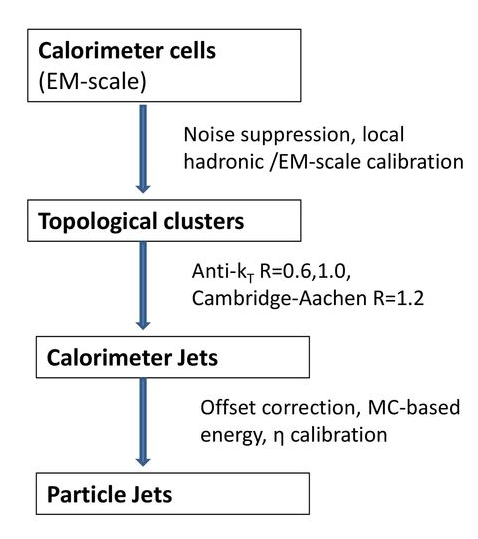
\includegraphics[width=0.6\textwidth]{jet-reconstruction}
  \caption{Jet Recontruction and Callibration Process}
\end{figure}

\subsubsection{Reconstruction:}
The recorded events then undergo reconstruction in large computing farms. Hits in the tracker are grouped and fitted into tracks. For example, in ATLAS the inner detector’s pixel and strip hits are first converted into 3D “space-points,” then combinatorially linked into track seeds and full helical fits. These tracks (momentum vectors) are then matched to calorimeter clusters to identify electrons, photons, muons, and charged hadrons.

Energy clusters in calorimeters (from electromagnetic or hadronic showers) are identified via clustering algorithms (e.g. sliding-window or “topo-cluster” methods) that collect adjacent cells above noise thresholds. Each event is thus reduced to a set of high-level physics objects (tracks, calorimeter jets, identified particle candidates) and derived observables (e.g. invariant masses, missing transverse energy, jet substructure). These analysis-ready datasets (often many gigabytes per run) are used for physics measurements and searches.


\subsection{Event Classification and Collision Regimes}


Collider data span a wide variety of event types. Proton–proton collisions at high energy typically produce events dominated by QCD jets and soft underlying activity. Experiments categorize events via trigger channels (e.g. single-muon triggers, dijet triggers, inclusive photon triggers, etc.).

Each category has different features and data rates. For instance, at CMS the full 40 MHz bunch-crossing rate yields many low-energy “minimum-bias” collisions, but the triggers preferentially record events with high-$p_T$ particles or large missing energy. Event properties vary strongly with beam conditions and collision systems.

\subsubsection{Using Hardware Triggers}

At high-luminosity proton runs (e.g. HL-LHC goals), pile-up dozens of simultaneous $\mathrm{pp}$ interactions per crossing creates events with hundreds of overlapping tracks and vertices, complicating reconstruction. By contrast, specialized runs (heavy-ion collisions or fixed-target setups) produce extremely high-multiplicity events.

\begin{figure}[H]
  \center
  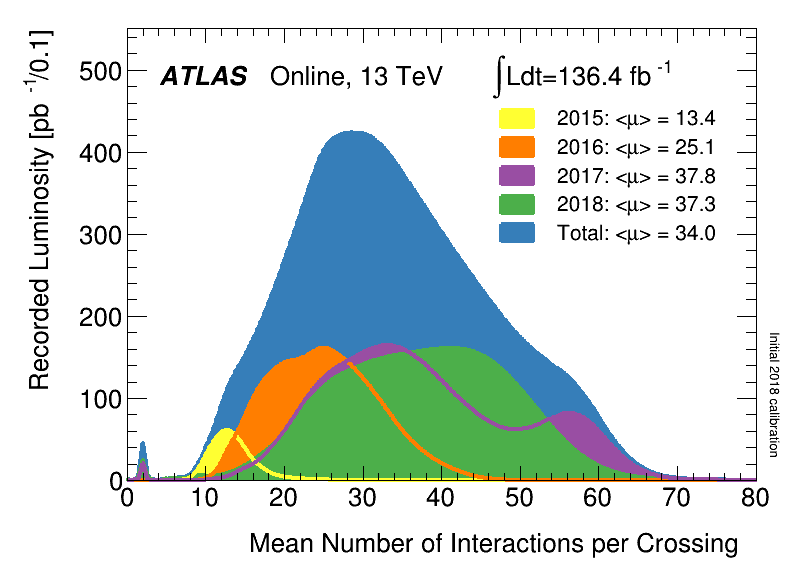
\includegraphics[width=0.6\textwidth]{hl}
  \caption{Mean number of interactions per bunch crossing for the ATLAS pp datasets }
\end{figure}

A striking example is the recent LHC heavy-ion program: in Run 3, ALICE recorded every Pb-Pb collision at 5.36 TeV/nucleon using continuous readout. This yielded $\sim1.2\times10^{10}$ lead-lead events (40× the previous total)
.

To handle this, ALICE deployed a 2800-GPU + 50k-CPU farm to process collisions at up to 770 GB/s throughput, compressing it to 170 GB/s for storage. In the end about 47.7 PB of disk data were collected from that run.

\subsubsection{Real-time Analysis}
This illustrates how collision regime (pp vs Pb-Pb) drives data rates and trigger strategy (e.g. no hardware trigger, just streaming and online compression). Other detectors reflect different geometries and physics goals.

For example, LHCb, a forward spectrometer for heavy-flavor physics, handles only a small fraction of LHC luminosity but implements a novel “real-time analysis” pipeline: Run 3 has no hardware trigger and reads out 40 MHz fully, using online reconstruction to compress data to ~10 GB/s written.

Thus LHCb can “cherry-pick” parts of each event (e.g. tracks from interesting decays) in real time. In contrast, ATLAS and CMS (general-purpose detectors) use multi-level triggers but now also deploy offline-style algorithms in their high-level triggers. Overall, events are classified by both physics (e.g. “dijet”, “vector boson”, “minimum bias”) and instrumental criteria (trigger signatures, pile-up conditions, beam type).

\begin{figure}[H]
  \center
  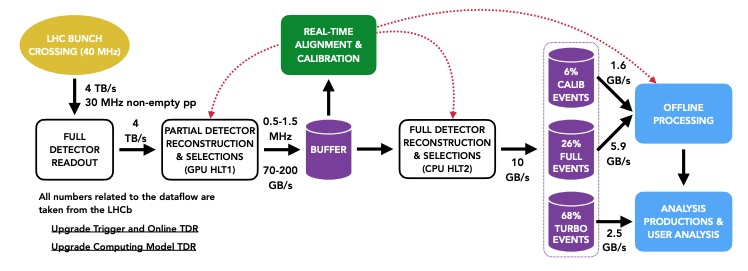
\includegraphics[width=0.9\textwidth]{lhcb}
  \caption{LHCb's realtime analysis frame work}
\end{figure}

Other detectors reflect different geometries and physics goals. For example, LHCb, a forward spectrometer for heavy-flavor physics, handles only a small fraction of LHC luminosity but implements a novel “real-time analysis” pipeline: Run 3 has no hardware trigger and reads out 40 MHz fully, using online reconstruction to compress data to ~10 GB/s written
. Thus LHCb can “cherry-pick” parts of each event (e.g. tracks from interesting decays) in real time. In contrast, ATLAS and CMS (general-purpose detectors) use multi-level triggers but now also deploy offline-style algorithms in their high-level triggers. Overall, events are classified by both physics (e.g. “dijet”, “vector boson”, “minimum bias”) and instrumental criteria (trigger signatures, pile-up conditions, beam type).

\section{Pipeline Bottlenecks and Technological Advances}

Despite improvements, critical bottlenecks remain. Trigger bandwidth is one: the fundamental limit is how much data can be read out and saved. Hardware triggers must decide in microseconds, and even HLT farms must process events at kHz–MHz rates. Experiments constantly upgrade trigger hardware: for Run 3, CMS installed 246 new servers with 25,600 CPU cores and 400 GPUs in its HLT farm

Software tools (e.g. hls4ml) are developing to put deep learning onto FPGAs for Level-1 triggers, enabling more intelligent real-time selection. Another bottleneck is simulation time. Detailed Monte Carlo (Geant4) simulation of particles through complex detectors is extremely CPU-intensive and often dominates computing budgets.

Machine learning offers a solution: generative models can accelerate simulation by orders of magnitude. For example, the CaloGAN framework uses GANs to simulate 3D calorimeter showers, achieving a 100-1000 times speedup on CPU and up to $~10^5$ times on GPU compared to full simulation
. Such techniques can produce high-fidelity synthetic data much faster, which is crucial as simulations are needed for virtually all analyses. (Challenges remain in covering the full physics phase space with adequate precision, but initial results are promising)


\section{Case Study: OpenData and ML Training Datasets}

The community has embraced open data: experiments now release large collision datasets for external research and ML development. CMS, for instance, has published over 2 PB of open proton–proton collision data (2010 Run1) under CC0 license
. ATLAS has released about 45 TB of 13 TeV data (7.1B events from 2015-16) in a lightweight analysis format
. These releases include reconstructed objects and sufficient metadata, though raw detector data (level-1) typically remains internal due to complexity.

Importantly, experiments now provide dedicated ML training samples. CMS’s latest open-data batch includes specialized ML datasets derived from millions of simulated events, each designed for core tasks: particle identification, track and vertex reconstruction, and pile-up (multiple-interaction) separation
cms.cern
. These samples come with full documentation and containerized analysis environments, enabling outsiders to apply state-of-the-art ML to realistic data. As Jesse Thaler (MIT) notes, “the performance of machine-learning techniques is directly tied to the quality of the underlying training data”
cms.cern
. By providing richly labeled, high-fidelity simulation samples, CMS (and similarly other experiments) allow researchers to develop and validate novel ML algorithms on collider-like datasets

\begin{table}[H]
  \centering
  \caption{Representative ML training datasets in High-Energy Physics as of 2022}
  \begin{tabular}{|p{2cm}|p{2.5cm}|p{2cm}|p{4cm}|p{3cm}|}
    \hline
    \textbf{Dataset} & \textbf{Source} & \textbf{Size} & \textbf{Target Tasks} & \textbf{Availability} \\
    \hline
    \textbf{CMS Open Data (2010 Run1)} & CMS Experiment & $\sim$2 PB (Raw + AOD) & Event classification, object ID, kinematic reconstruction & Public, via CERN OpenData portal \\
    \hline
    \textbf{ATLAS Open Data (13 TeV)} & ATLAS Experiment & $\sim$45 TB & Physics object analysis, event selection, jet tagging & Public, curated formats \\
    \hline
    \textbf{CaloGAN / CaloDiffusion} & Simulated (Calorimeter geometry) & $\sim$GBs & Fast simulation of calorimeter showers using generative models & Public, via GitHub + Zenodo \\
    \hline
    \textbf{TrackML Challenge} & Simulated (ATLAS-like detector) & $\sim$200 GB & Track reconstruction using GNNs / Hough transform & Public, via CERN + Kaggle \\
    \hline
    \textbf{HEPML (CMS ML datasets)} & CMS, curated for ML & $\sim$10–100 GB (varies) & Pile-up mitigation, particle ID, energy regression & Public, CMS OpenData (ML repo) \\
    \hline
    \textbf{LHC Olympics 2020/2021} & Simulated (LHC backgrounds + new physics) & $\sim$10–50 GB & Unsupervised anomaly detection, signal discovery & Public, via website \\
    \hline
    \textbf{Higgs Kaggle Challenge (2014)} & Simulated (ATLAS-based) & $\sim$50 MB & Signal vs background classification for Higgs-like events & Public, via Kaggle repository \\
    \hline
    \textbf{Open Lorentz Datasets} & Theoretical models (e.g. EFT, jets) & 1–20 GB & Jet tagging, event generation from theory models & Public, from physics ML groups \\
    \hline
  \end{tabular}
  \label{tab:hepml_datasets}
\end{table}



\subsubsection{Adressing the Simulation and Real Gap}

However, drawbacks remain. Simulated training data (though plentiful) can suffer from the “simulation–real gap”: physics models and detector simulators are approximate, and ML models trained purely on MC may not generalize perfectly to real data. Conversely, real collision data have no truth labels, making supervised training difficult. To mitigate this, analyses often use mixed datasets: e.g. train on MC but calibrate or fine-tune on data control samples. Generative ML offers another remedy: for example, GAN-based fast simulators like CaloGAN (above) can be trained on real detector responses to produce synthetic examples that bridge some of this gap. In summary, building robust ML models typically requires combining multiple sources – real data, full simulation, and ML-generated data – to fully capture the physics and detector variability


\section{Conclusion}
High-energy physics has transformed data science: from isolated MB experiments to continuous petabyte-scale streams demanding global grids and AI tools. Every collision generates multi-gigabyte detector readouts, which must be quickly filtered, reconstructed, and distilled into physics insights. As data rates rise (via HL-LHC and future colliders), the field is pushing new frontiers in computing: real-time triggers without hardware limits
, GPU-accelerated reconstruction
, and ML-driven simulation and analysis
. Preserving and exploiting these data require careful pipeline design and a rich ecosystem of datasets. Emerging ML methods, supported by open and simulated data, promise to help overcome current bottlenecks and may reshape the path from collision to discovery in the coming decades.

\end{spacing}
\end{document}
